% \begin{figure*}[tp] 
% \vspace{-0. in}
% \centering
% \centerline{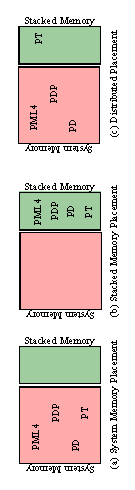
\psfig{file=FIGURES/pagetable_placement,scale=0.80,angle=-90,width=\textwidth}}
% \caption{\small Different page table placement policies in a hybrid
% 	memory system. \normalsize}
% \label{fig:pagetable_placement} 
% \vspace{-0.0in}
% \end{figure*}

%\newpage
\begin {table}[h]
\begin{center} 
\vspace{-0.1in}
\caption{Baseline System Configuration}
\vspace{-0. in}
\begin{tabular}{|c|c|}
\hline
     \multicolumn{2}{|c|}{Streaming Multiprocessor (SM)}               \\ \hline
     Frequency            &  1 GHz                                    \\ 
     Number of SMs        &  128                                        \\ \hline
     \multicolumn{2}{|c|}{Baseline TLB and Cache Hierarchy}            \\ \hline
     L1 TLB   (private)   &  32-entry, 4-way                \\ 
     L2 TLB   (shared)    &  1024-entry, 8-way            \\ \hline
     L1 cache (private)   &  128KB,  4-way, 128B linesize  \\ 
     L2 Cache (shared)    &  8MB, 16-way, 128B linesize \\
     MSHRs for Mem Reqs   &  128 per memory channel  \\ \hline
     \multicolumn{2}{|c|}{Stacked Memory (HBM)}            \\ \hline
     Capacity             &  16GB (4 stacks)          \\
     Bus Frequency        &  1 GHz     \\ 
     Channels / Banks    &  32  / 16 per rank        \\
     Bus Width            &  128-bits per channel    \\ 
     Row Buffer Size      &  2048 Bytes              \\
     \small{tCAS-tRCD-tRP-tRAS}   &  14-14-14-33     \\ 
     Total Bandwidth      &  1024 GB/s              \\ \hline
     \multicolumn{2}{|c|}{Main Memory (DDR4)}               \\ \hline
     Capacity             &  256GB                   \\
     Bus Frequency        &  1600MHz (DDR 3.2GHz)    \\ 
     Channels / Banks    &  8  / 16 per rank        \\
     Bus Width            &  64 bits per channel     \\ 
     Row Buffer Size      &  2048 Bytes              \\
     \small{tCAS-tRCD-tRP-tRAS}   &  14-14-14-35     \\ 
     Total Bandwidth      &  204.8 GB/s               \\ \hline
     \multicolumn{2}{|c|}{Virtual Memory Configuration}     \\ \hline
%      ATS Lookup Latency   &  50 ns (oneway) \\
     Page Allocation      &  BW-aware Placement~\cite{batman,bwa}  \\ 
     Page Table (PT)      &  4-level hierarchical    \\ 
     Page Walk Caches     &  16 entries per PT level       \\ \hline

\end{tabular}
\label{table:method_system}
\vspace{-0.3in}
\end{center}
\normalsize
\end{table}


\section{Experimental Methodology}
\label{sec:method}

\noindent We assume a CPU-GPU heterogeneous system (see
Figure~\ref{fig:config}) with a single CPU and a single GPU supporting
shared virtual memory~\cite{intelgen9, amdzen, gpu_pascal}. We assume
GPU LLT misses are serviced by sending address translation service
(ATS) ~\cite{vesley2016ispass,ats_spec} requests to the CPU IOMMU.

\subsection{System Configuration}

\noindent We use an industry proprietary performance simulator to
simulate a GPU (Table~\ref{table:method_system}) with a memory
hierarchy based on the NVIDIA Pascal GPU system~\cite{gpu_pascal}. We
model 128 Streaming Multiprocessors (SM) that support 64 warps each. A
warp scheduler selects warp instructions each cycle. The baseline GPU
memory system consists of a multi-level cache and TLB hierarchy. The
first-level cache and TLB are private to each SM while the last-level
cache (LLC) and last-level TLB (LLT) are shared by all the
SMs~\cite{SharedLLT}. All caches use 128B cache line size with 32B
sectors. We assume 5 bytes of tag storage per LLC entry (including
valid, dirty, coherence state, and replacement bits). For the UCAT
architecture, we assume an extra 40 cycle load-to-use latency to
consult the UCAT on an LLT miss. The baseline LLC (and UCAT) use the
DRRIP replacement policy~\cite{jaleel_rrip} while the L1 cache and
TLBs use pseudo-LRU replacement~\cite{jaleel_rrip}.

% Each TLB supports compressing up to four contiguous TLB
% entries into a single entry~\cite{COLT}. 

We model a hybrid memory subsystem consisting of 16GB of High
Bandwidth Memory (HBM) technology~\cite{hbm-spec} (referred to as
stacked memory) and 256GB of commodity DRAM (referred to as system
memory) using conventional DDR4 technology~\cite{ddr4-spec}. The
stacked memory has 5$x$ the bandwidth of system memory with similar
random access latency. To ensure full utilization of the total
available system bandwidth, physical pages are allocated based on the
bandwidth ratio of the hybrid memory system~\cite{bwa,batman}. In
doing so, both system memory and stacked memory satisfy memory
requests. The CPU and GPU have similar interconnect latency to the
system memory controller and stacked memory controller (50ns in both
cases). The memory controller supports 128-entry read and write queues
per channel, open-page policy, minimalist address mapping
policy~\cite{minimalist} and FR-FCFS scheduling policy (prioritizing
reads over writes). Writes are issued in batches when the write queue
starts to fill up.

% This isolates our performance studies to the bandwidth capability of
% the two memory systems rather than the latency to and from each
% individual memory system. We discuss performance implications with
% different interconnect latency (e.g. discrete CPU/GPU systems) in
% Section~\ref{sec:implications}.

We model a virtual memory system that maps virtual addresses to
physical addresses using random page replacement. Our baseline assumes
4KB page size, however we also study sensitivity to larger page size.
We model a four-level hierarchical page table~\cite{SkipPT}: Page Map
Level 4 (PML4), Page Directory Pointer (PDP), Page Directory (PD), and
Page Table (PT). All application pages tables reside in system memory.
To speed up address translation, we model on-chip Page Walk Caches
(PWCs)~\cite{SkipPT, MMUcaches} for each page table level. The PWCs
are small, fully associative hardware structures that are indexed by
portions of the virtual address and are co-located on-chip with the
MMUs~\cite{MMUcaches}. We model a 16-entry PML4-cache, 16-entry
PDP-cache, a 16-entry PD-cache, and a 16-entry
PT-cache\cite{MMUcaches}. Finally, we assume a highly-threaded
hardware page table walker for handling misses in the
PWCs~\cite{power2014supporting, pichaigpu}.

\subsection{Workloads and Metric of Interest}

\noindent We use selected CUDA-based high performance computing
applications from CORAL~\cite{CORAL}, Mantevo~\cite{mantevo}, and
LoneStar~\cite{lonestar} suites (see Table~\ref{table:bench_char}). We
also CUDA versions of a graph-traversal workload
($MaxFlow$~\cite{maxflow})) and a random memory access workload
($GUPS$~\cite{gups}). The workloads are all run with large inputs to
stress the hybrid memory system. We collected representative program
regions and warm up the caches, TLBs, and PWCs by executing four
billion warp instructions. After functional warmup, we enable detailed
timing simulation for two billion warp instructions.

Reduction in total execution time is our primary metric for
performance. We also compare virtual to physical address translation
latency to correlate the change in performance. We compute translation
latency as the cycles spent in translating a virtual address to
physical address averaged across all memory instructions executed by
the application.

% collect average LLT miss latency. The reduction in LLT miss latency
% directly correlates with performance improvements, we
